\chapter{\Large Réalisation}

\textbf{\huge Introduction} \\[1cm]

Au cours de ce dernier chapitre, on va exposer le travail accompli, explorer les différentes étapes pour réaliser le travail final en détaillant chaque étape et en incluant quelques captures d'écran expliquant le processus de déploiement de la solution. \\[0.1cm]
\section{\fontfamily{ptm}\selectfont\Large  Environnement de travail }
Dans cette partie, nous présentons les environnements matériels et logiciels utilisés dans le
cadre de notre projet.
\subsection{\fontfamily{ptm}\selectfont\Large  Environnement matériel }
Au cours de les différentes étape de notre projet, nous avons disposé de deux PC ayant les
caractéristiques suivantes(voir tableau 3.1) :
\begin{center}
    \begin{table}[H]  
      \centering
      \resizebox{1\textwidth}{!}{
  \begin{tabular}{|c|c|c|}
  \hline
    \textbf{Marque} &  \textbf{lenovo ideapad 3} & \textbf{Lenovo Legion slim 7} \\
  \hline
  \textbf{Processeur} & \textbf{AMD Rayzen 5 3.3GHZ} & \textbf{AMD Rayzen 9 4.10GHZ} \\
  \hline
  \textbf{Mémoire Vive} & \textbf{16GB RAM} & \textbf{16GB RAM} \\
  \hline
  \textbf{Stockage}& \textbf{500GB} & \textbf{1To}  \\
  \hline
  \textbf{Systéme d'exploitation }& \textbf{Fedora 37} &\textbf{Windows 11}\\
  \hline
  \end{tabular}
  }
  \caption{Caractéristiques des ordinateurs}
  \end{table}
  \end{center}
  \subsection{\fontfamily{ptm}\selectfont\Large Architecture technologique globale}
   Dans cette partie nous allons présenter l'architecture globale de notre projet(voir figure 3.1).
\begin{landscape}
  \begin{figure}[htbp]
    \centering
  \includegraphics[width=25cm,height=17cm]{GLOBALAWS.png}  
    \caption{Architecture globale}
  \end{figure}
\end{landscape}
  \subsection{\fontfamily{ptm}\selectfont\Large  Environnement Logiciel }
  Dans cette partie, nous présentons les environnements logiciels différents utilisés.(voir tableau 3.2)
  \subsubsection{\fontfamily{ptm}\selectfont\Large  Environnement et technologie de développement }
  \newcolumntype{C}[1]{>{\centering\arraybackslash}p{#1}}
  \begin{center}
    \begin{table}[H]  
      \centering
      %\resizebox{0.8\textwidth}{!}{
  \begin{tabular}{|m{5cm}|m{5cm}|m{5cm}|}
  \hline
    \textbf{Nom} &  \textbf{Description} & \textbf{Utilisation} \\
  \hline
  \centering
\includegraphics[width=3cm,height=3cm]{autre_partie/VSCODE.png}   & \textbf{Visual Studio Code est un éditeur de code source développé par Microsoft.} & \textbf{Nous avons utilisé Visual studio code pour la développement de code et interagi avec github.} \\
  \hline
\centering
\includegraphics[width=2cm,valign=c]{autre_partie/VMW.png}&\textbf{VMware Workstation est un outil de virtualisation de poste de travail créé par la société VMware, il peut être utilisé pour mettre en place un environnement de test pour développer de nouveaux logiciels, ou pour tester l'architecture complexe d’un système d’exploitation avant de l’installer réellement sur une machine physique.\cite{21} }& \textbf{Nous avons utilisé Vmware pour créer diffèrent virtual machine pour deployée le cluster.} \\
\hline
\centering
\includegraphics[width=4cm,valign=c]{autre_partie/Latex.png}&\textbf{Latex est un logiciel de préparation de documents qui utilise le programme de composition TeX pour formater sa sortie, et est lui-même écrit dans le langage de macro TeX. Le latex est largement utilisé dans les universités pour la publication de documents scientifiques dans de nombreux domaines, y compris les mathématiques, l’informatique, etc.}& \textbf{Nous avons utilisé Latex pour rédaction de notre rapport.} \\
  \hline
  \centering
\includegraphics[width=2cm,valign=c]{autre_partie/GitHub-Logo.png}& \textbf{Github est un site développé par Chris Wanstrath, PJ Hyett et Tom Preston-Werner. Fournir divers services qui aident les développeurs à gérer leur code source à l'aide du logiciel de gestion de versions Git.} & \textbf{Nous avons utilisé Github pour déposer notre code.}  \\
  \hline
  \centering
\includegraphics[width=2cm,valign=c]{autre_partie/Docker-Symbol.png}& \textbf{Docker est une plate-forme qui rend l’exécution, le test et la livraison de logiciels plus rapide avec sa virtualisation au niveau OS qui permet de séparer l’application dans des conteneurs.} &\textbf{Nous avons utilisé docker dans la création des images docker.}\\
  \hline

  \end{tabular}
  %}
  \end{table}
  \end{center}
  \newpage
  \begin{center}
    \begin{table}[H]  
      \centering
      %\resizebox{0.8\textwidth}{!}{
  \begin{tabular}{|m{5cm}|m{5cm}|m{5cm}|}
  \hline
  \centering
\includegraphics[width=3cm,valign=c]{autre_partie/github-actions.png}& \textbf{GitHub Actions est une plateforme CI/CD (Continuous Integration and Continuous Delivery) qui vous permet d'automatiser votre pipeline de construction, de test et de déploiement. Vous pouvez créer des flux de travail qui construisent et testent chaque requête merge ,pull ou push sur votre dépôt.} & \textbf{Nous avons utilisé Github Action  pour la création et l'exécution de notre pipeline.}  \\
  \hline
  \centering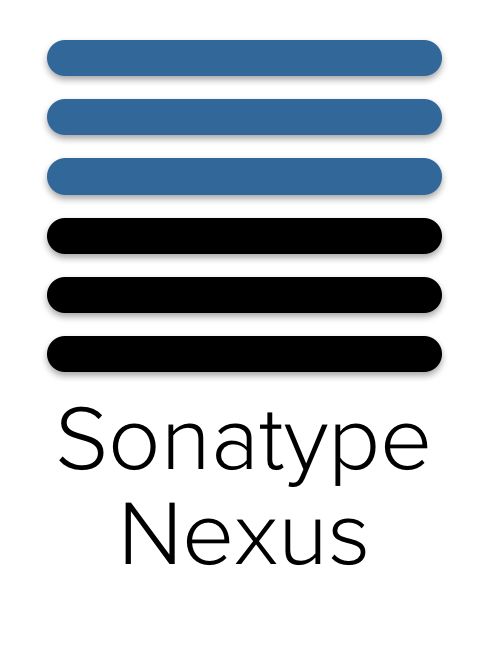
\includegraphics[width=3cm,valign=c]{autre_partie/Nexus.png}& \textbf{Nexus est gestionnaire de dépôt qui vous permet de proxy, collecter et gérer différents artefacts et image docker et rendre facile de distribuer votre logiciel. } & \textbf{Nous avons utilisé Nexus pour gérer notre artefact de l'application développer.}  \\
  \hline
  \centering
\includegraphics[width=3cm,valign=c]{autre_partie/SONARQ.png}& \textbf{sonarqube est une plateforme open source développée par SonarSource pour le contrôle de code qualité et les rapports de code statique, elle supporte différents langages et frameworks de programmation. } & \textbf{Nous avons utilisé Sonarqube pour l'analyse de notre code source et vérifier la présence des défauts.}  \\
  \hline
  \centering
\includegraphics[width=3cm,valign=c]{autre_partie/ANSIBLE.png}& \textbf{Ansible est un outil d’automatisation qui fournit une infrastructure en tant que code créé par Michael DeHaan et acquit par Red Hat, il fournit des outils pour la configuration, le déploiement d’application et le provisionnement. } & \textbf{Nous avons utilisé Ansible pour automatiser la configuration de cluster local et les ressources cloud.}  \\
  \hline
\centering
\includegraphics[width=4cm,valign=c]{autre_partie/K8s.png}& \textbf{Kubernetes est un système open source qui automatiser le déploiement, la mise à l’échelle et la gestion des applications dans des conteneurs} & \textbf{Nous avons utilisé Kubernetes pour la déploiement des diffèrent application et outils.}  \\
\hline
\centering
\includegraphics[width=3cm,valign=c]{autre_partie/prometheus-logo-png-transparent.png}& \textbf{Prometheus est un système open source développé par soundcloud pour la collection de données et de métriques à l’aide d’un modèle http pull. } & \textbf{Nous avons utilisé Prometheus pour la collection des diffèrent données des outils,clusters et applications.}  \\
\hline
\centering
\includegraphics[width=2cm,valign=c]{autre_partie/grafana-logo.png}& \textbf{Grafana est une application Web d’analyse open source et visualisation interactive. Il fournit des graphiques et des alertes lorsqu’il est connecté à des sources de données prises en charge. } & \textbf{Nous avons utilisé Grafana pour la création des alerts et visualisation des diffèrent données collecter par prometheus en forme des différent diagrammes.}  \\
\hline

  \end{tabular}
  %}
  \end{table}
  \end{center}
  \begin{center}
    \begin{table}[H]  
      \centering
      %\resizebox{0.8\textwidth}{!}{
  \begin{tabular}{|m{5cm}|m{5cm}|m{5cm}|}
  \hline
\centering
\includegraphics[width=4cm,valign=c]{autre_partie/Slack_RGB.png}& \textbf{Slack est un logiciel de messagerie développé par Slack Technologies.Slack est développé pour les communications professionnelles et organisationnelles. } & \textbf{Nous avons utilisé Slack pour recevoir les alert créer par Grafana.}  \\
\hline
\centering
\includegraphics[width=4cm,valign=c]{autre_partie/EKS.png}& \textbf{EKS is a service to create a managed kubernetes cluster by amazon it offers different add-ons that help to interact with other services like EBS,ALB or NLB. } & \textbf{Nous avons utilisé EKS pour créer un cluster pour l'environnement de production.}  \\
\hline
\centering
\includegraphics[width=3cm,valign=c]{autre_partie/ECR.png}& \textbf{Amazon elastic container Registry (Amazon ECR) est un service qui registre les images docker dans des répertoires soit public soit privé. } & \textbf{Nous avons utilisé ECR pour enregistrer notre diffèrent image docker.}  \\
\hline
\centering
\includegraphics[width=4cm,valign=c]{autre_partie/EC2.png}& \textbf{EC2 (Elastic Compute Cloud) est un serivce fourni par amazon faire facile aux utilisateurs de louer des ordinateurs virtuels pour exécuter leurs propres applications. } & \textbf{Nous avons utilisé EC2 pour créer des noued pour le cluster EKS.}  \\
\hline
\end{tabular}
%}
\caption{Environnement et technologies de développement}
\end{table}
\end{center}
  \subsection{\fontfamily{ptm}\selectfont\Large  Langage Informatique }
  \textsf{\fontfamily{ptm}\selectfont\scalefont{1.3} Le tableau ci-dessous répresente les diffèrents langage utilisé dans le projet.}  
  \newcolumntype{C}[1]{>{\centering\arraybackslash}p{#1}}
  \begin{center}
    \begin{table}[H]  
      \centering
      %\resizebox{0.8\textwidth}{!}{
  \begin{tabular}{|m{5cm}|m{5cm}|m{5cm}|}
  \hline
    \textbf{Nom} &  \textbf{Description} & \textbf{Utilisation} \\
  \hline
\centering
\includegraphics[height=2cm,width=2cm]{autre_partie/ReactJs.png}   & \textbf{React js est une bibliothèque open source utilisée pour construire des interfaces, il peut également être utilisé sur IOS, Android et web } & \textbf{Cette langage est utilisée dans l'application qui nous avons testé dans notre projet.} \\
  \hline
  \centering
\includegraphics[width=2cm,valign=c]{autre_partie/yaml.png}&\textbf{YAML (Ain’t Markup Language) un langage de sérialisation de données développé par Clark Evans, Ingy döt Net et Oren Ben-Kiki, utilisé pour créer des fichiers de configuration.}& \textbf{Nous avons utilisé ce langage pour créer différent playbooks. } \\
  \hline
\end{tabular}
%}
\caption{Langage informatique}
\end{table}
\end{center}
\subsection{\fontfamily{ptm}\selectfont\Large  Environnement de Conception}
\textsf{\fontfamily{ptm}\selectfont\scalefont{1.3} Le tableau ci-dessous répresente les diffèrents outil de conception utilisé dans le projet.}  
\newcolumntype{C}[1]{>{\centering\arraybackslash}p{#1}}
\begin{center}
  \begin{table}[H]  
    \centering
    %\resizebox{0.8\textwidth}{!}{
\begin{tabular}{|m{5cm}|m{5cm}|m{5cm}|}
\hline
  \textbf{Nom} &  \textbf{Description} & \textbf{Utilisation} \\
\hline
\centering
\includegraphics[width=2cm,valign=c]{autre_partie/Draw.png}   & \textbf{draw.io est une application de source libre qu'il est utiliser pour illustrer des diagrammes. } & \textbf{Ce outil est utilisée pour les différents diagrammes dans notre projet.} \\
\hline
\centering
\includegraphics[width=4cm,valign=c]{autre_partie/Canva-Logo.png}&\textbf{Canva est un outil de conception graphique en ligne gratuit,utiliser pour créer des présentations, des logos et plus encore}& \textbf{Nous avons utilisé canva pour désigner quelque diagrammes. } \\
\hline
\end{tabular}
%}
\caption{Environnement de conception}
\end{table}
\end{center}
\section{\fontfamily{ptm}\selectfont\Large Sprint1 :Configuration de l'architecture cloud}
\textsf{\fontfamily{ptm}\selectfont\scalefont{1.3} Pour ce partie nous allons configuré tout les ressources cloud que nous besoin pour la projet.}
\subsection{\fontfamily{ptm}\selectfont\Large  Configuration des ressources cloud}
\textsf{\fontfamily{ptm}\selectfont\scalefont{1.3} Pour la configuration des ressources cloud nous avons préparer un playbook ansible qui créer les ressources nécessaire dans AWS comme VPC,Subnets,route,security groups,EKS and ECR.ou début en definit les différent variables pour les ressources}
\begin{figure}[H]
    \begin{center}
    \fbox{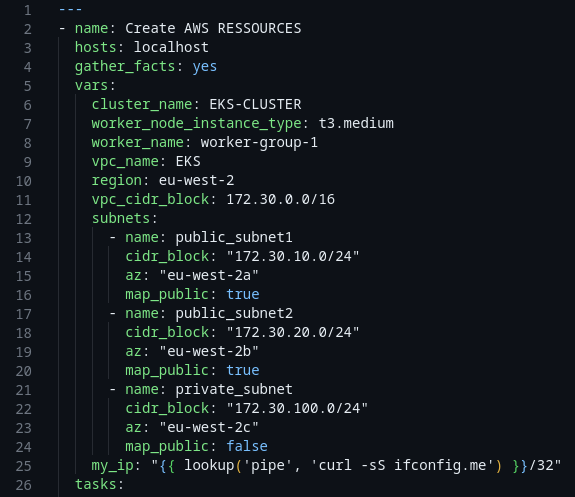
\includegraphics[height=10cm,width=10cm]{autre_partie/VARS.png}}
    \end{center}
    \caption{Les variables de playbook ansible}
    \end{figure}
    \textsf{\fontfamily{ptm}\selectfont\scalefont{1.3}Aprés la définition des variable dans le playbook on passe a les tâches qui sera exécuter par Ansible:\\
    \indent
     
\begin{tikzpicture}
        \draw[fill=black] (2,2) circle (2pt);
      \end{tikzpicture} Tâche << Créer VPC >>:
      \begin{figure}[H]
        \begin{center}
        \fbox{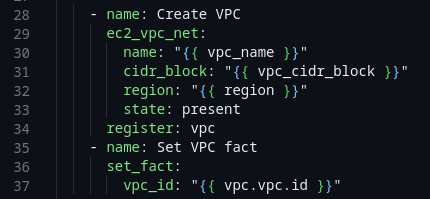
\includegraphics[width=10cm]{VPC.png}}
        \end{center}
        \caption{Tâche de VPC} 
        \end{figure}
        \indent
        
\begin{tikzpicture}
           \draw[fill=black] (2,2) circle (2pt);
         \end{tikzpicture} Tâche << Créer les sous-réseaux >>:
         \begin{figure}[H]
           \begin{center}
           \fbox{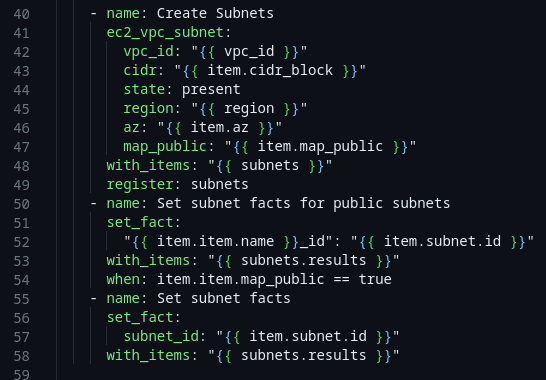
\includegraphics[width=10cm]{SUBNETS.png}}
           \end{center}
           \caption{Tâche des sous-réseaux}
           \end{figure}
           \indent
           
\begin{tikzpicture}
              \draw[fill=black] (2,2) circle (2pt);
            \end{tikzpicture} Tâche << Créer passerelle Internet >>:
            \begin{figure}[H]
              \begin{center}
              \fbox{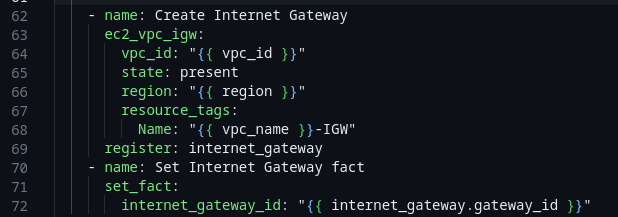
\includegraphics[width=11cm]{IGW.png}}
              \end{center}
              \caption{Tâche de passerelle internet}
              \end{figure}
              \indent
              
\begin{tikzpicture}
                 \draw[fill=black] (2,2) circle (2pt);
               \end{tikzpicture} Tâche << Créer route >>:
               \begin{figure}[H]
                 \begin{center}
                 \fbox{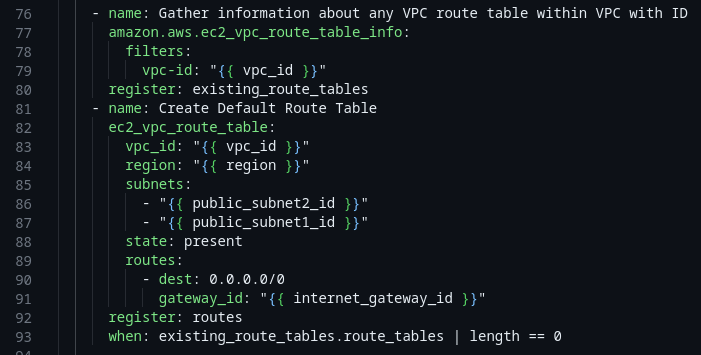
\includegraphics[width=11cm]{ROUTE.png}}
                 \end{center}
                 \caption{Tâche de route internet}
                \end{figure}
                \indent
                
\begin{tikzpicture}
                   \draw[fill=black] (2,2) circle (2pt);
                 \end{tikzpicture} Tâche << Créer la sécurite groupe >>:
                 \begin{figure}[H]
                   \begin{center}
                   \fbox{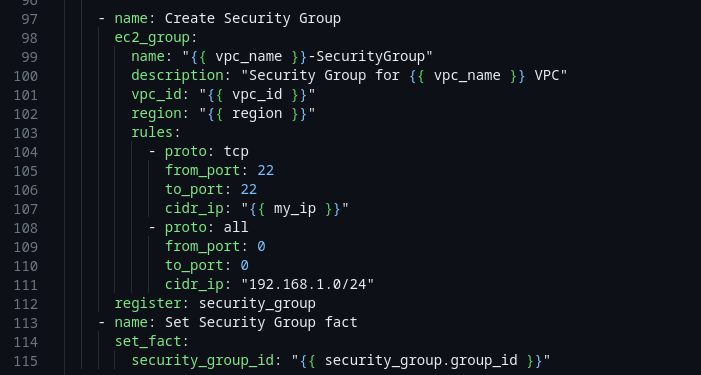
\includegraphics[width=11cm]{SECURITYGR.png}}
                   \end{center}
                   \caption{Tâche de sécurité groupe.}
                  \end{figure}
                  \indent
                  
\begin{tikzpicture}
                     \draw[fill=black] (2,2) circle (2pt);
                   \end{tikzpicture} Tâche << Créer EKS cluster >>:
                   \begin{figure}[H]
                     \begin{center}
                     \fbox{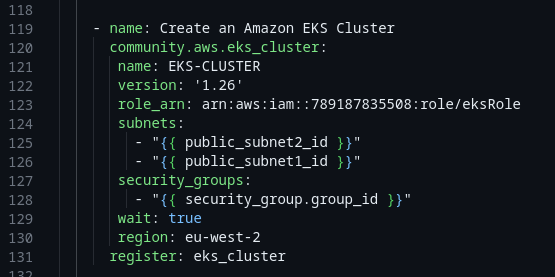
\includegraphics[width=11cm]{EKSCL.png}}
                     \end{center}
                     \caption{Tâche de cluster EKS.}
                    \end{figure}
                    \indent
                    
\begin{tikzpicture}
                       \draw[fill=black] (2,2) circle (2pt);
                     \end{tikzpicture} Tâche << Créer Noeud de travail pour le cluster EKS >>:
                     \begin{figure}[H]
                       \begin{center}
                        \fbox{ 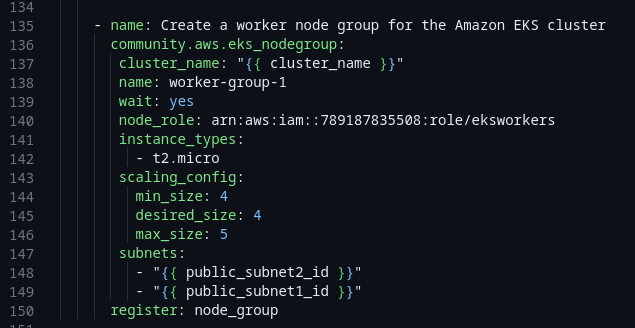
\includegraphics[width=11cm]{WORKERNODES.png}}
                       \end{center}
                       \caption{Tâche de noeud de travail.}
                      \end{figure}
                      \indent
                      
\begin{tikzpicture}
                         \draw[fill=black] (2,2) circle (2pt);
                       \end{tikzpicture} Tâche << Créer répertoire ECR >>:
                       \begin{figure}[H]
                         \begin{center}
                            \fbox{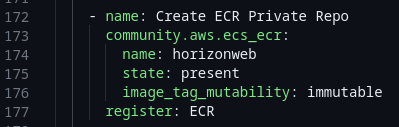
\includegraphics[width=11cm]{ECRPH.png}}
                         \end{center}
                         \caption{Tâche de ECR}
                        \end{figure}
                        \indent
                        
\begin{tikzpicture}
                           \draw[fill=black] (2,2) circle (2pt);
                         \end{tikzpicture} Résultat de l'execution de playbook (voir figure 5.10):
                         \begin{figure}[H]
                           \begin{center}
                              \fbox{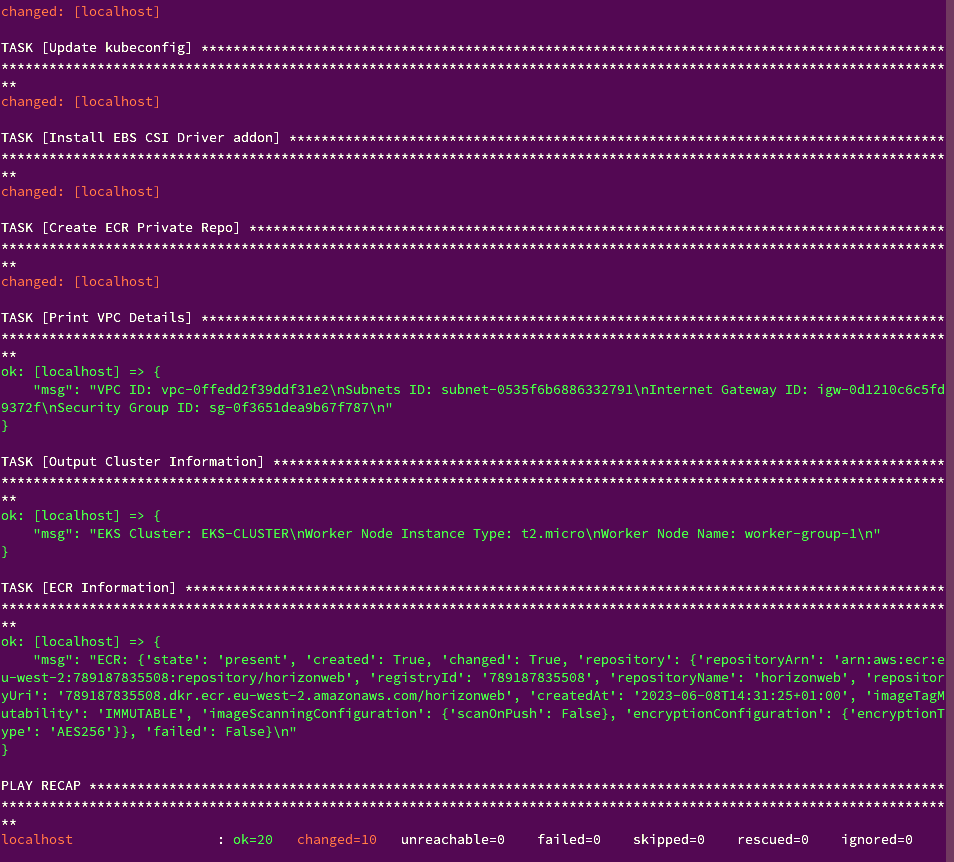
\includegraphics[width=17cm,height=13cm]{EKSRESPUP.png}}
                           \end{center}
                           \caption{Résultat de playbook.}
                          \end{figure}
                          }   
%%%%%%%%%%%%%%%%%%%%%%%%%%%%%%%%%%%%%%%%%%%ADDDDDDDDDDDDDDDDDDDDD_RESULTATSSSSSSSSSSSSSSSSSSSSSSSSSSSSS%%%%%%%%%%%%%%%%%%%%%%%%%%%%%%%%%%%%%%%
\subsection{\fontfamily{ptm}\selectfont\Large  Configuration de cluster local}
\textsf{\fontfamily{ptm}\selectfont\scalefont{1.3} Pour ce partie nous allons configuré tout les ressources local que nous besoin pour la projet.}
\subsubsection{\fontfamily{ptm}\selectfont\Large  Provisionnement de les machines virtuelles}
\textsf{\fontfamily{ptm}\selectfont\scalefont{1.3} Nous allons configuré les machines virtuelles pour enfin installer le cluster local et déployé les outils nécessaire pour la fonctionnement de projet.\\

\begin{tikzpicture} 
    \draw[fill=black] (2,2) circle (2pt);
  \end{tikzpicture} La création des virtuelles machines sera faite avec Vmware Workstation (voir figure 5.11)
  \begin{figure}[H]
    \begin{center}
       \fbox{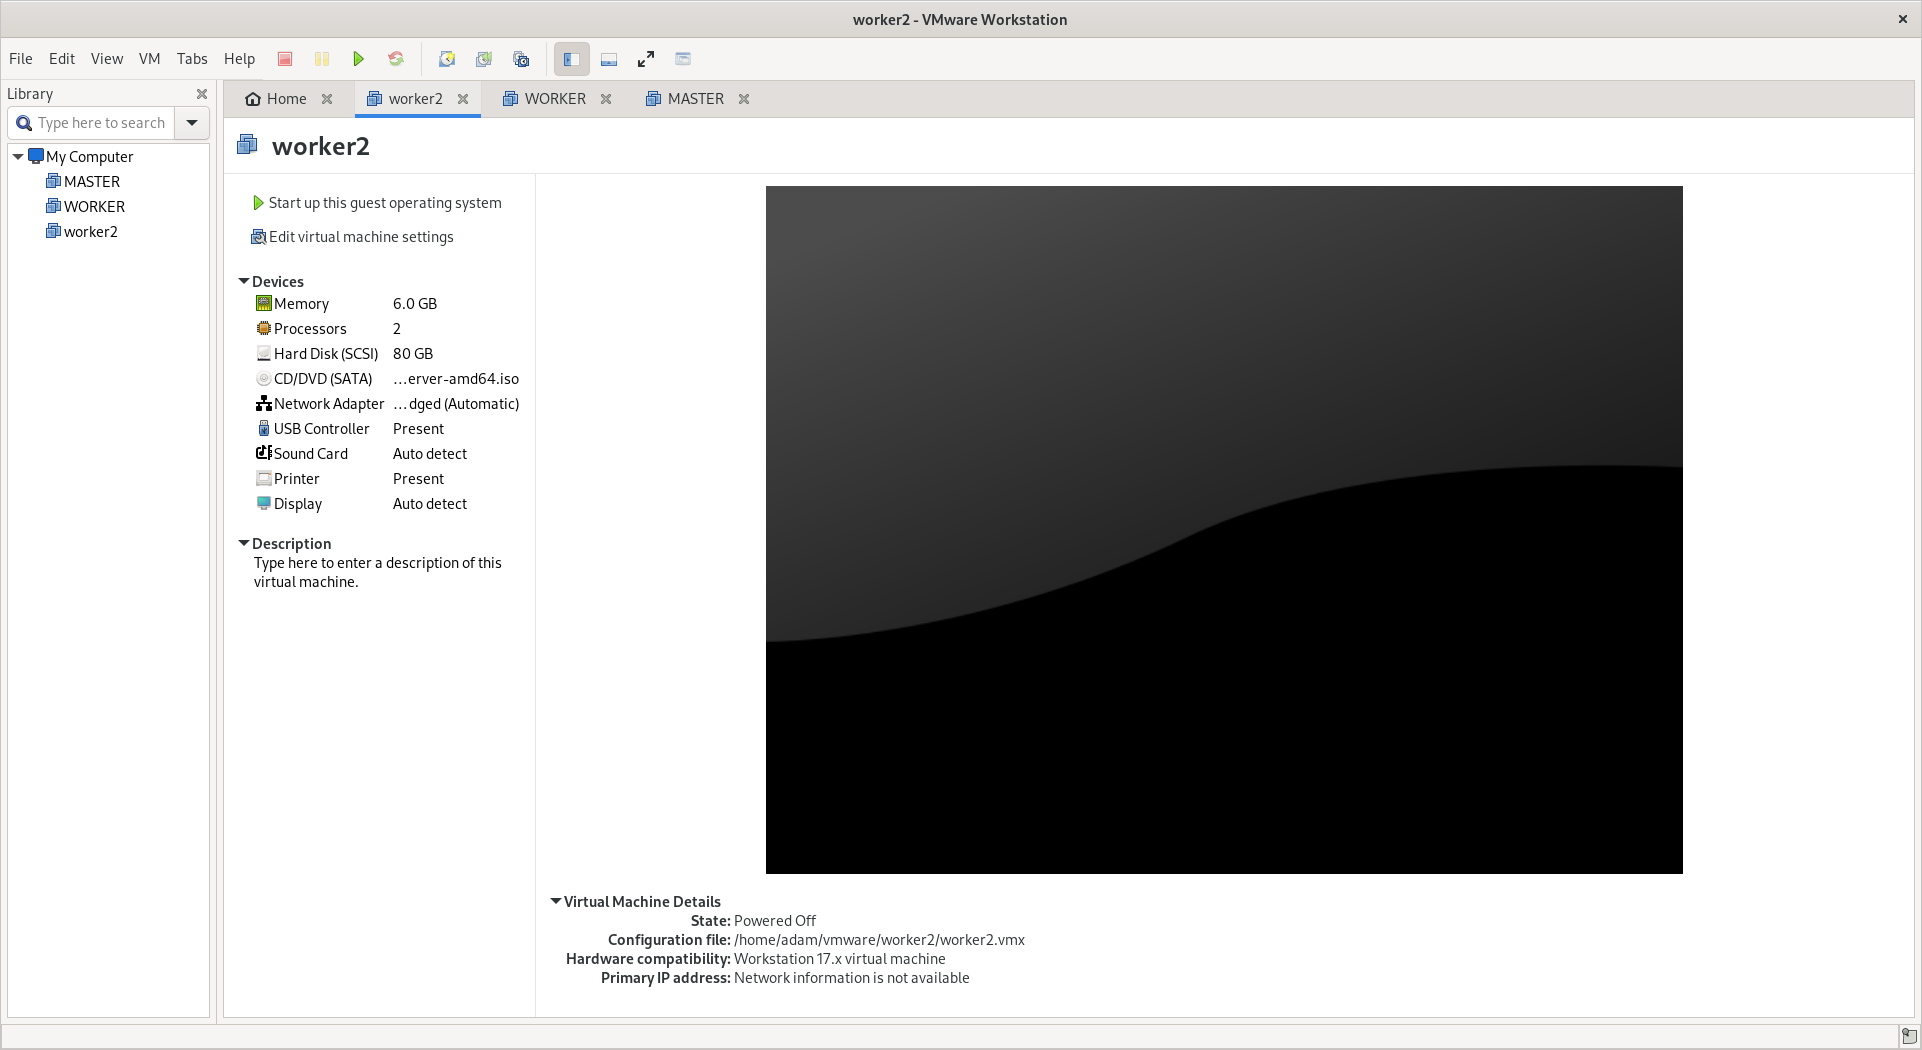
\includegraphics[width=18cm]{VM.png}}
    \end{center}
    \caption{Les machines virtuelles.}
   \end{figure}
Pour la configuration de cluster nous avons utilisé Ansible pour l'optimisation du temps:\\

\begin{tikzpicture} 
    \draw[fill=black] (2,2) circle (2pt);
  \end{tikzpicture} L'installation des logiciels nécessaire sera fait avec ansible on exécutent le playbook "Configuration.yaml" sur les machines virtuelles.(voir figure 5.12, 5.13 et 5.14)
  \begin{figure}[H]
    \begin{center}
       \fbox{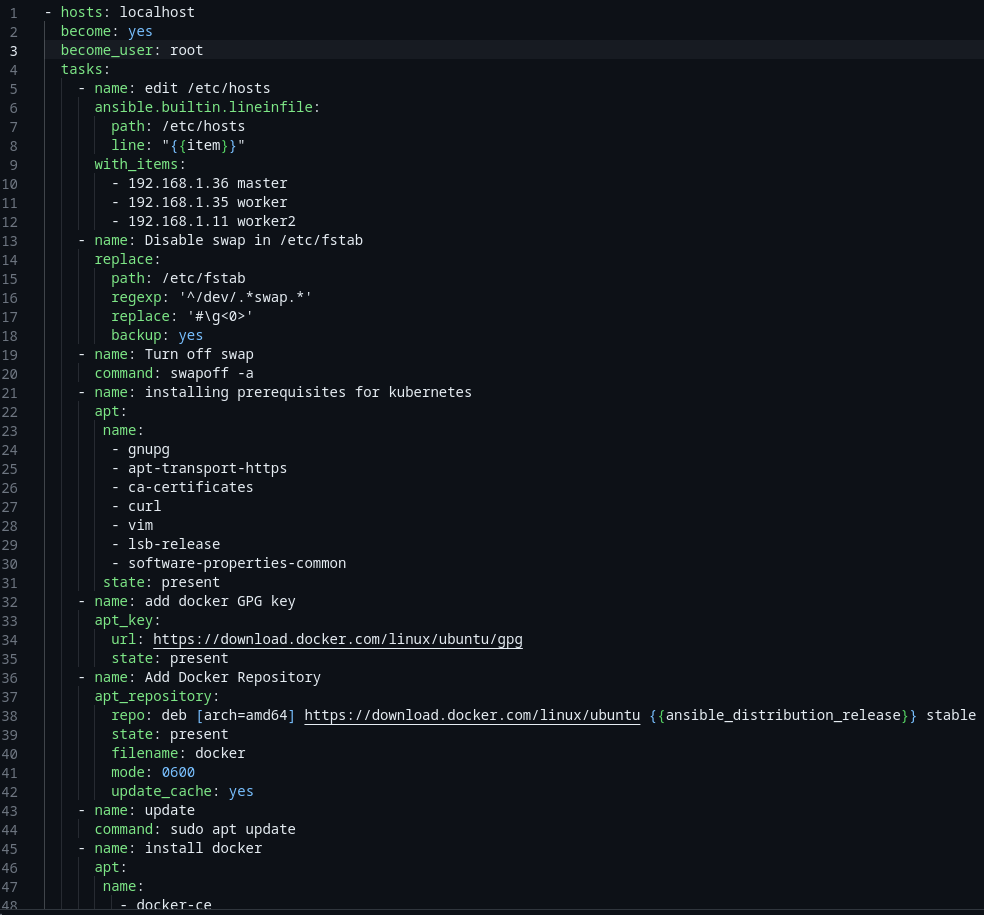
\includegraphics[width=17cm,height=13cm]{installer.png}}
    \end{center}
    \caption{Playbook Ansible d'installation(1).}
   \end{figure}
   \begin{figure}[H]
    \begin{center}
       \fbox{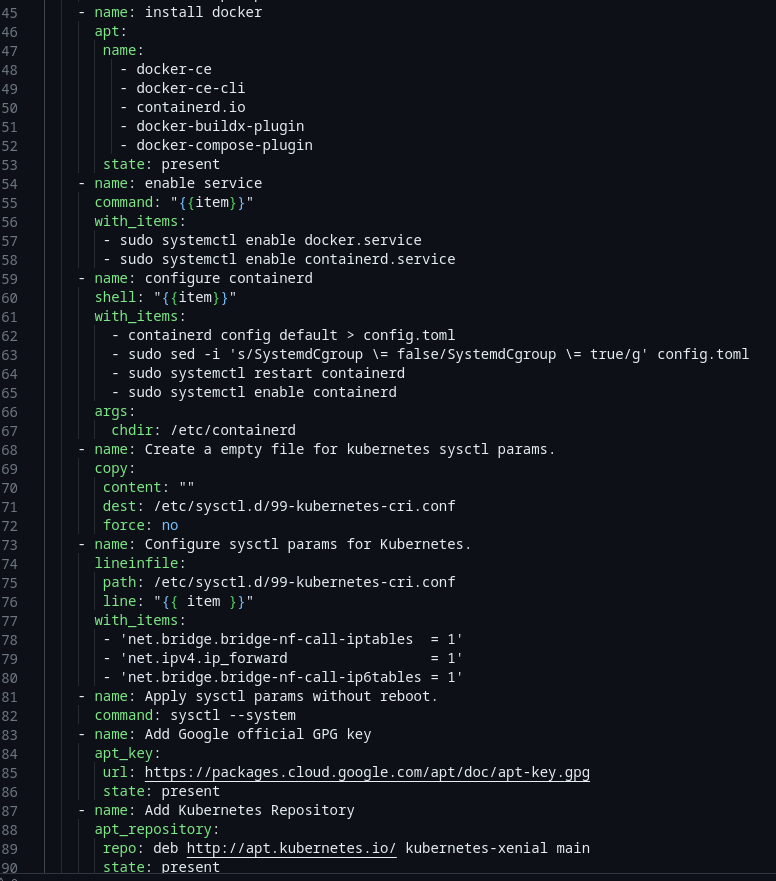
\includegraphics[width=10cm,height=15cm]{installer2.png}}
    \end{center}
    \caption{Playbook Ansible d'installation(2).}
   \end{figure}
   \begin{figure}[H]
    \begin{center}
       \fbox{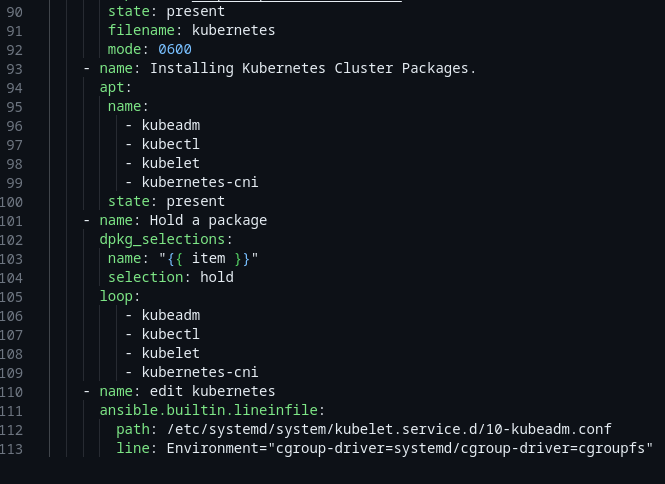
\includegraphics[width=10cm,height=15cm]{installer3.png}}
    \end{center}
    \caption{Playbook Ansible d'installation(3).}
   \end{figure}
   \indent\indent Le résultat de l'exécution de ce playbook aprés le commande "ansible-playbook Configuration.yaml"(voir figure 5.15)
   \begin{figure}[H]
    \begin{center}
       \fbox{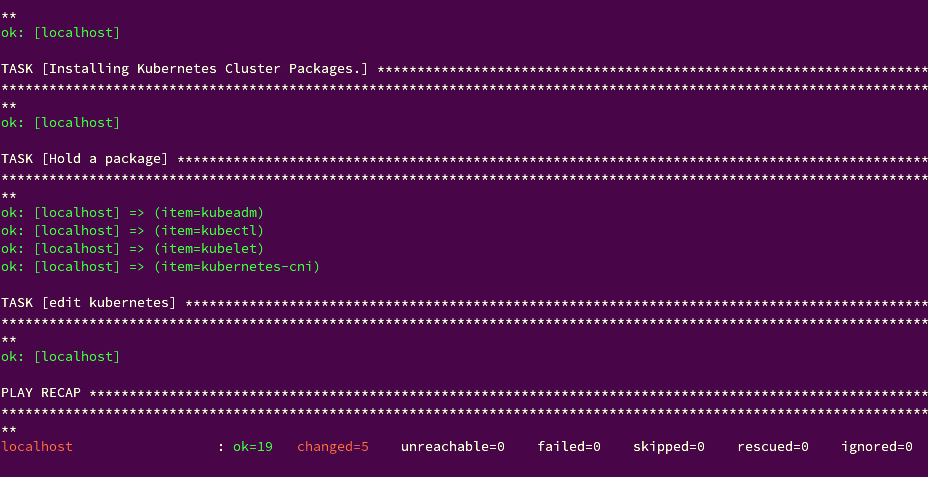
\includegraphics[width=17cm,height=9cm]{resultatwhit.png}}
    \end{center}
    \caption{résultat d'installation.}
   \end{figure}
   
\begin{tikzpicture} 
    \draw[fill=black] (2,2) circle (2pt);
  \end{tikzpicture} Aprés l'installation, la configuration de la machine master sera fait avec playbook "ConfigMaster.yaml"(voir figure 5.156
   \begin{figure}[H]
    \begin{center}
       \fbox{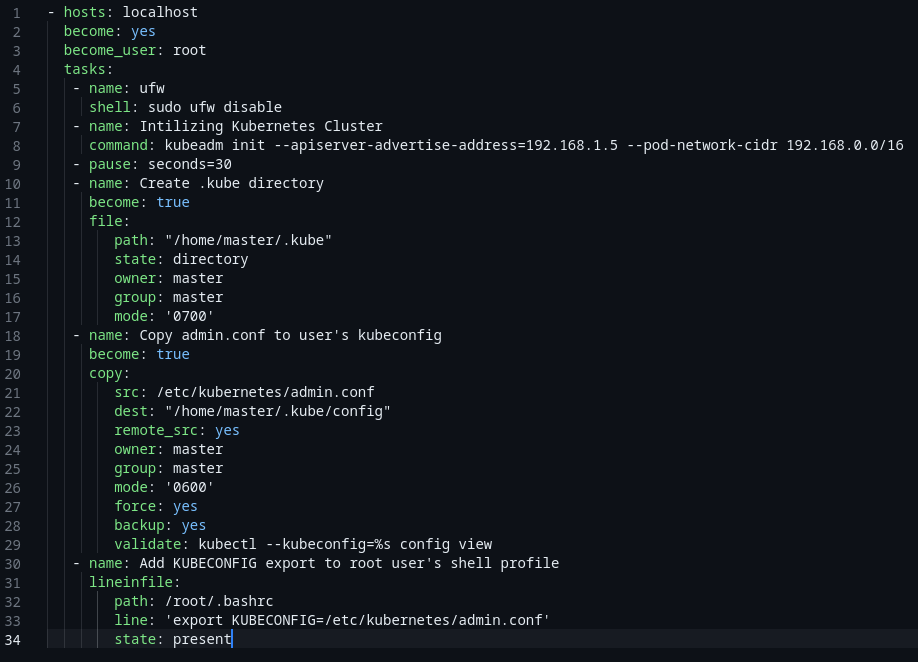
\includegraphics[width=10cm,height=13cm]{Conf.png}}
    \end{center}
    \caption{playbook Configuration de master.}
   \end{figure}
    \indent\indent Résultats de l'exécution de la playbook "ConfigMaster.yaml" (voir figure 5.17)
    \begin{figure}[H]
        \begin{center}
           \fbox{\includegraphics[width=17cm,height=12cm]{CONF.png}}
        \end{center}
        \caption{Résultat de playbook "ConfigurationMaster.yaml".}
       \end{figure} 
       
\begin{tikzpicture} 
        \draw[fill=black] (2,2) circle (2pt);
      \end{tikzpicture} Le cluster requis une configuration de réseau pour la communication entre les noeuds et les pods pour configurer le réseau nous avons préparer un playbook "NetworkPolicy.yaml" (voir figure 5.18)
       \begin{figure}[H]
        \begin{center}
           \fbox{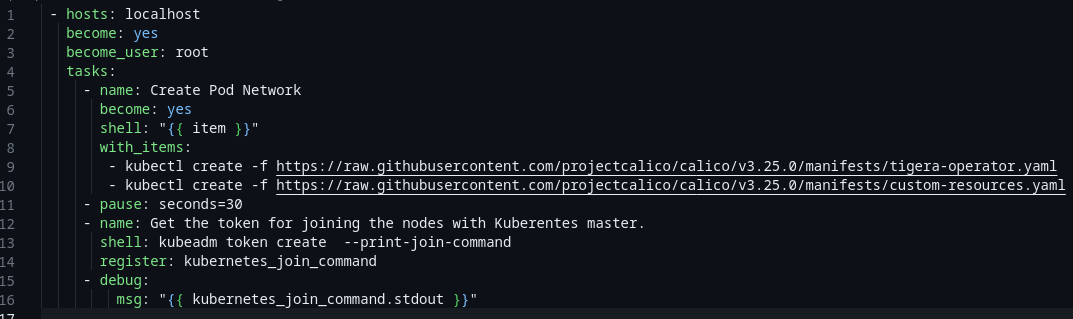
\includegraphics[width=18cm,height=9cm]{Network.png}}
        \end{center}
        \caption{playbook NetworkPolicy.yaml.}
       \end{figure}
       \indent\indent Résultats de l'exécution de la playbook "NetworkPolicy.yaml" (voir figure 5.19)
       \begin{figure}[H]
           \begin{center}
              \fbox{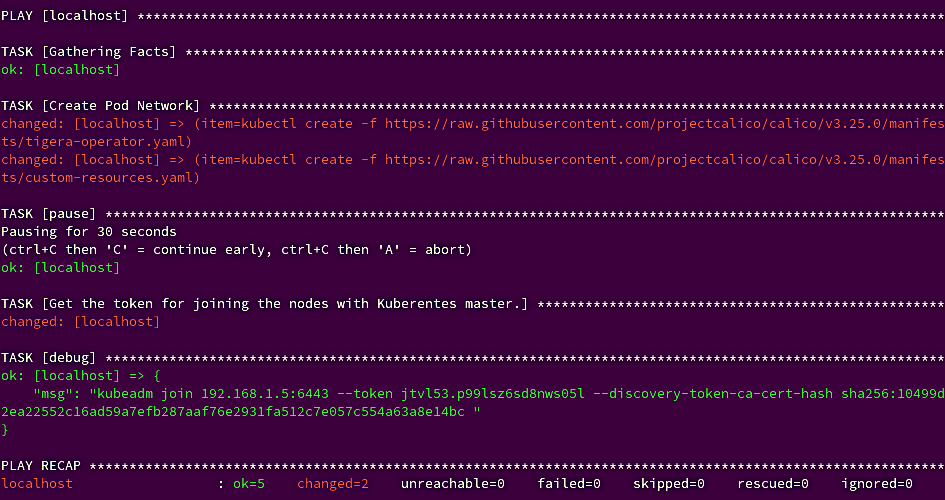
\includegraphics[width=18cm,height=12cm]{NetworkWHITE.png}}
           \end{center}
           \caption{Résultat de playbook "NetworkPolicy.yaml".}
          \end{figure} 
          
\begin{tikzpicture} 
            \draw[fill=black] (2,2) circle (2pt);
        \end{tikzpicture} Aprés la configuration de calico dans le cluster l'ingénieur DevOps exécute la commande "Kubeadm join" qui est afficher aprés l'exécution de playbook "NetworkPolicy.yaml", dans les noeud qui nous avons créé comme des noeuds du travail.(voir figure 5.19 pour le commande "Kubeadm join").\\Enfin la cluster local est prét(voir figure 5.20)
        \begin{figure}[H]
         \begin{center}
            \fbox{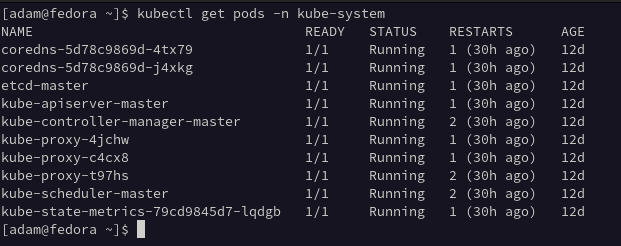
\includegraphics[width=15cm,height=10cm]{CLUSTERLOCAL.png}}
         \end{center}
         \caption{Cluster locale.}
        \end{figure}
         }
         \subsubsection{\fontfamily{ptm}\selectfont\Large  Configuration de Sonarqube}
         \textsf{\fontfamily{ptm}\selectfont\scalefont{1.3} Nous allons configuré et déployé SonarQube sur notre cluster pour analyse la qualité de notre code .\\
         
\begin{tikzpicture} 
             \draw[fill=black] (2,2) circle (2pt);
           \end{tikzpicture} Pour déployé SonarQube il faut créer les diffèrent fichier nécessaire (voir figure 5.21)
           \begin{figure}[H]
             \begin{center}
                \fbox{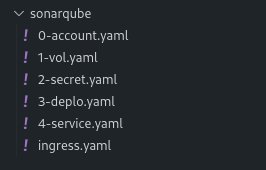
\includegraphics[width=8cm]{SONARFILES.png}}
             \end{center}
             \caption{Liste des fichier (SonarQube).}
            \end{figure}
            \indent\indent Ces fichier sont déployé aprés l'exécution de commande:\\\indent\indent "kubectl apply -f ./sonarqube -n sonarqube" (voir figure 5.22)
            \begin{figure}[H]
                \begin{center}
                   \fbox{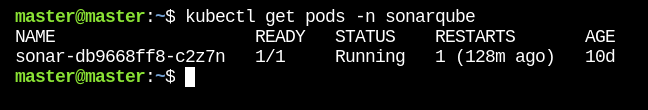
\includegraphics[width=14cm]{SONAKUBE.png}}
                \end{center}
                \caption{Pod SonarQube.}
               \end{figure}      
               \indent\indent La figure suivante présente l'interface de SonarQube (voir figure 5.23)
               \begin{figure}[H]
                   \begin{center}
                      \fbox{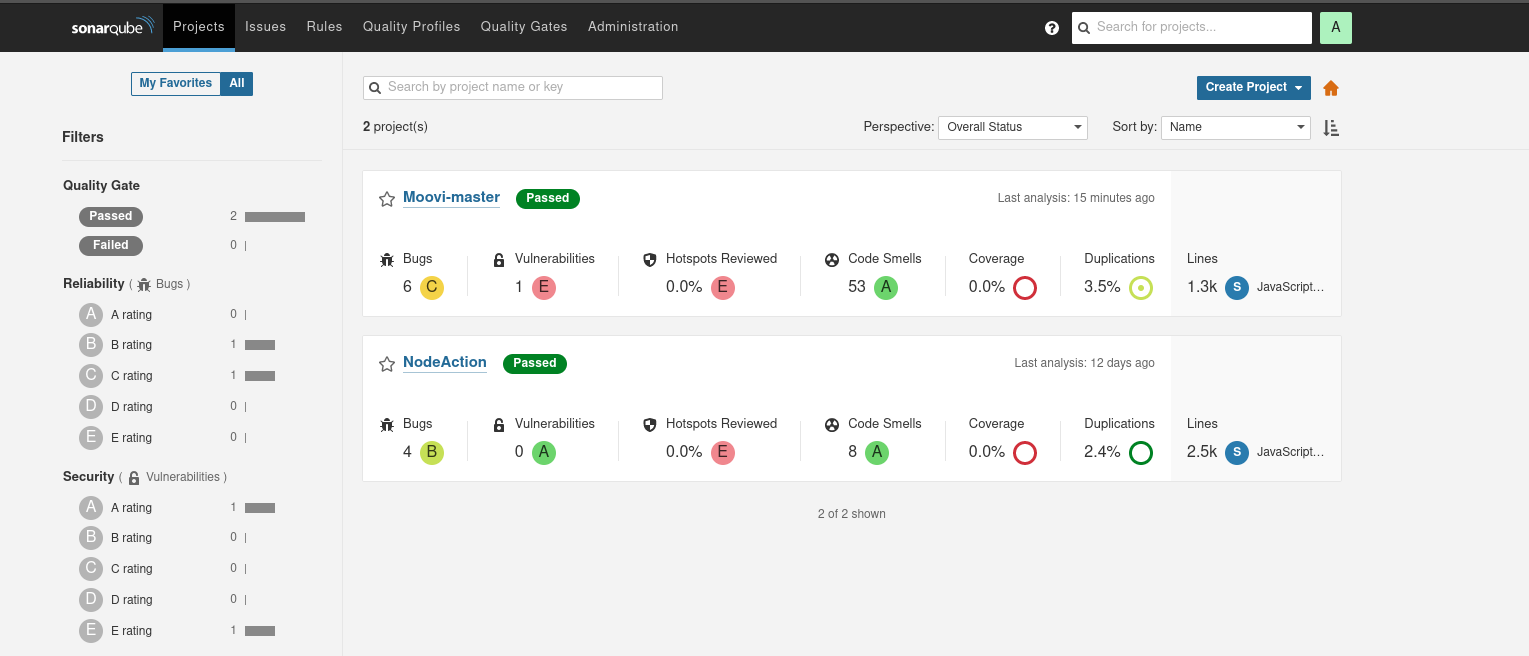
\includegraphics[width=18cm]{SONARINTERFACE.png}}
                   \end{center}
                   \caption{Interface de SonarQube.}
                  \end{figure}             
         }
         \subsubsection{\fontfamily{ptm}\selectfont\Large  Configuration de Nexus}
         \textsf{\fontfamily{ptm}\selectfont\scalefont{1.3} Nous allons configuré et déployé Nexus sur notre cluster stocker les artefacts de notre code.\\
         
\begin{tikzpicture} 
             \draw[fill=black] (2,2) circle (2pt);
           \end{tikzpicture} Pour déployé Nexus il faut créer les diffèrent fichier nécessaire (voir figure 5.24)
           \begin{figure}[H]
             \begin{center}
                \fbox{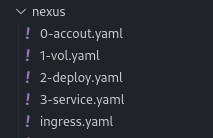
\includegraphics[width=7cm]{NEXUSFILES.png}}
             \end{center}
             \caption{Liste des fichier (Nexus).}
            \end{figure}
            \indent\indent Ces fichier sont déployé aprés l'exécution de commande:\\\indent\indent "kubectl apply -f ./nexus -n nexus" (voir figure 5.25)
            \begin{figure}[H]
                \begin{center}
                   \fbox{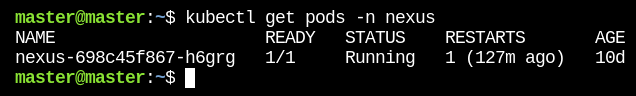
\includegraphics[width=14cm]{NEXUSKUBE.png}}
                \end{center}
                \caption{Pod Nexus.}
               \end{figure} 
               \indent\indent La figure suivante présente l'interface de Nexus (voir figure 5.26):
               \begin{figure}[H]
                   \begin{center}
                      \fbox{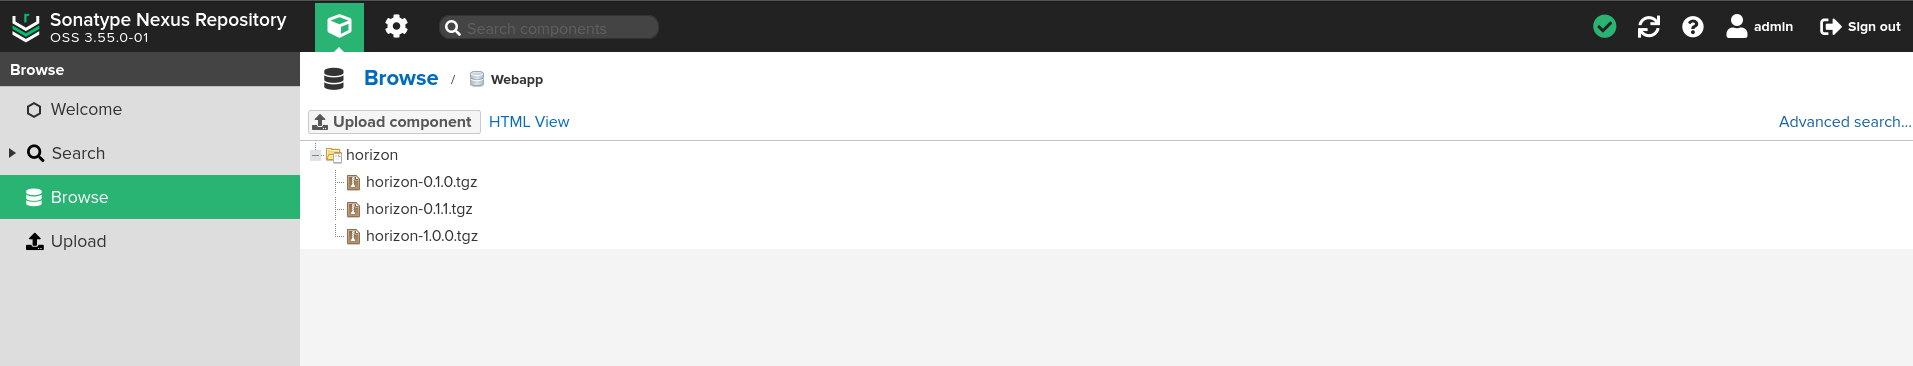
\includegraphics[width=18cm]{NEXUSINTERFACE.png}}
                   \end{center}
                   \caption{Interface de Nexus.}
                  \end{figure} 
         }
         \subsubsection{\fontfamily{ptm}\selectfont\Large  Outils des surveillances}
         \textsf{\fontfamily{ptm}\selectfont\scalefont{1.3}\\
         
\begin{tikzpicture} 
             \draw[fill=black] (2,2) circle (2pt);
           \end{tikzpicture} Pour déployé les outils des surveillances il faut créer les diffèrent fichier nécessaire (voir figure 5.27)
           \begin{figure}[H]
             \begin{center}
                \fbox{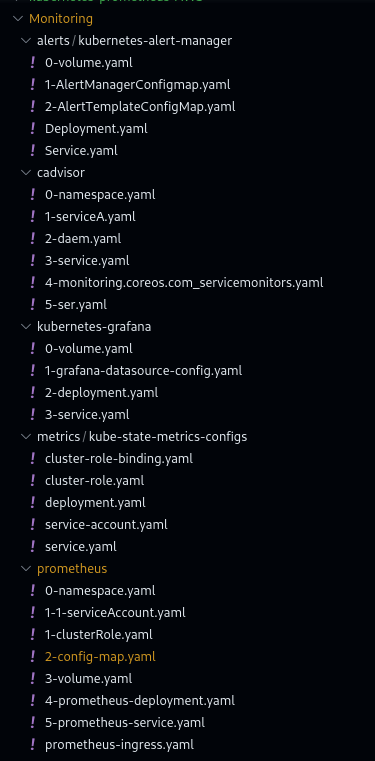
\includegraphics[width=7cm]{MONITORING.png}}
             \end{center}
             \caption{Liste des fichier (Monitoring).}
            \end{figure}
            \indent\indent Ces fichier sont déployé aprés l'exécution de commande:\\\indent\indent "kubectl apply -f ./Monitoring -n monitoring"(voir figure 5.28)
            \begin{figure}[H]
                \begin{center}
                   \fbox{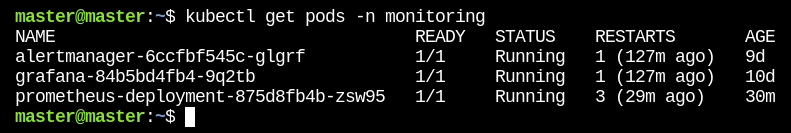
\includegraphics[width=15cm]{MONIKUBE.png}}
                \end{center}
                \caption{Les Pods de namespace Monitoring.}
               \end{figure} error: unable to upgrade connection: container not found ("grafana")
                }
\section{\fontfamily{ptm}\selectfont\Large Sprint2 :Configuration de pipeline}
\textsf{\fontfamily{ptm}\selectfont\scalefont{1.3} Pour ce partie nous allons configuré les workflow qui sont lancer quand une changement dans notre code est détecter.}
\subsection{\fontfamily{ptm}\selectfont\Large  Création des pipelines}
\textsf{\fontfamily{ptm}\selectfont\scalefont{1.3} Configuration de pipeline pour les différent branches:\\

\begin{tikzpicture} 
    \draw[fill=black] (2,2) circle (2pt);
  \end{tikzpicture} Pipeline de branche Main (voir figure 5.29 et 5.30)
  \begin{figure}[H]
    \begin{center}
       \fbox{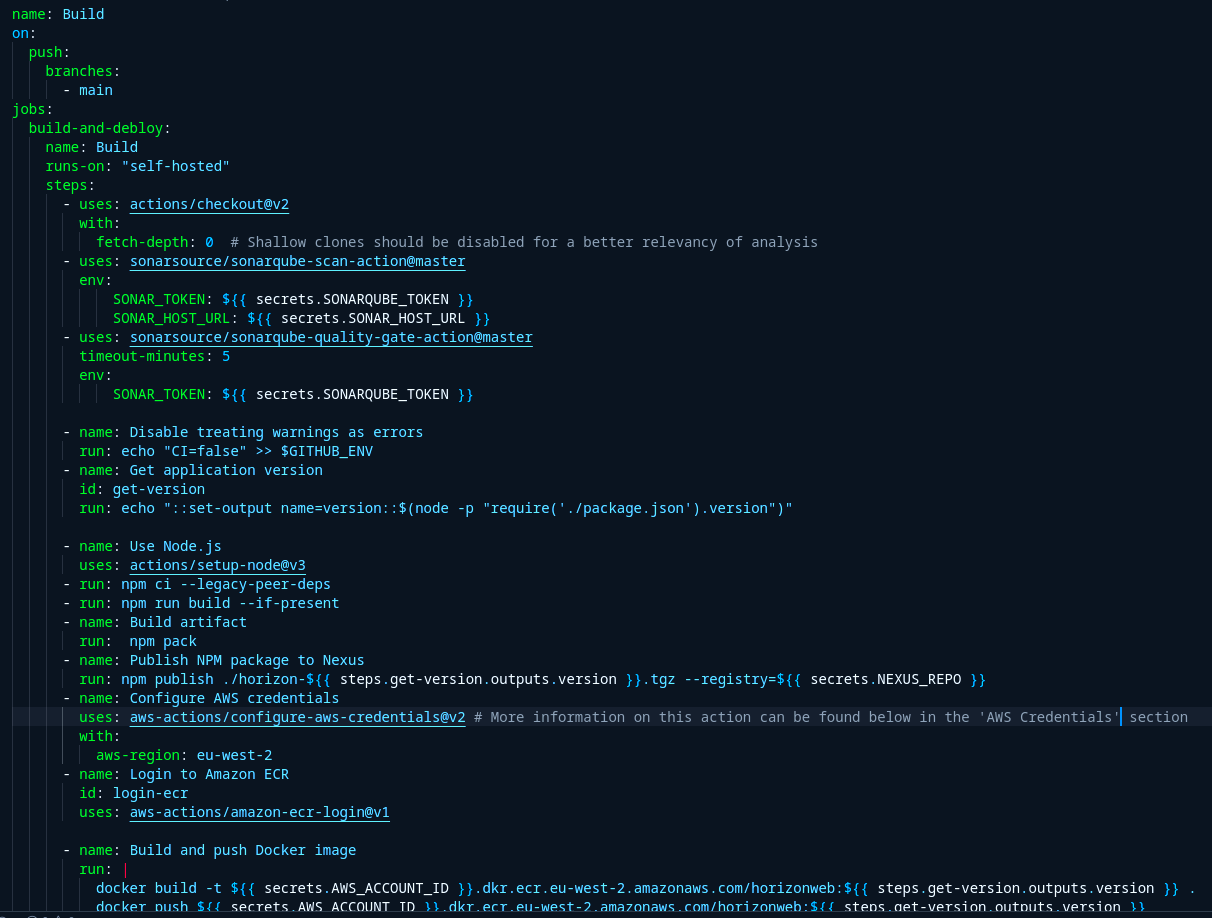
\includegraphics[width=17cm,height=12cm]{PIPE111.png}}   
    \end{center}
    \caption{Pipeline de branche main(1).}
   \end{figure}
     \begin{figure}[H]
    \begin{center}
       \fbox{\includegraphics[width=17cm,height=12cm]{PIPE121.png}}
    \end{center}
    \caption{Pipeline de branche main(2).}
   \end{figure}
   \indent\indent Encore de la lancement de la pipeline différent action sera exécuter (voir figure 5.31)
   \begin{figure}[H]
       \begin{center}
          \fbox{\includegraphics[width=10cm,height=12cm]{GITA1.png}}
       \end{center}
       \caption{Github Action interface.}
      \end{figure}
      
\begin{tikzpicture} 
        \draw[fill=black] (2,2) circle (2pt);
      \end{tikzpicture} Pipeline de branche EKS (voir figure 5.32 et 5.33)
      \begin{figure}[H]
        \begin{center}
           \fbox{\includegraphics[width=18.5cm,height=13cm]{PIPE211.png}}   
        \end{center}
        \caption{Pipeline de branche EKS(1).}
       \end{figure}
         \begin{figure}[H]
        \begin{center}
           \fbox{\includegraphics[width=18cm,height=9cm]{PIPE222.png}}
        \end{center}
        \caption{Pipeline de branche EKS(2).}
       \end{figure}
       \indent\indent Encore de la lancement de la pipeline différent action sera exécuter (voir figure 5.34)
       \begin{figure}[H]
           \begin{center}
              \fbox{\includegraphics[width=10cm,height=12cm]{GITA2.png}}
           \end{center}
           \caption{Github Action interface.}
          \end{figure}
}
\subsection{\fontfamily{ptm}\selectfont\Large  Configuration d'exécuteur local }
\textsf{\fontfamily{ptm}\selectfont\scalefont{1.3} Pour ce partie nous allons configuré l'exécuteur qui exécuter les workflows de notre projet.(voir figure 5.35)}
\begin{figure}[H]
    \begin{center}
       \fbox{\includegraphics[width=18cm]{RUNNER.png}}
    \end{center}
    \caption{Github Action Runner.}
   \end{figure}
   \textsf{\fontfamily{ptm}\selectfont\scalefont{1.3} Aprés l'exécution d'un pipeline l'application sera deployé dans l'environnement corespond a la besoin.\\
   
\begin{tikzpicture} 
      \draw[fill=black] (2,2) circle (2pt);
    \end{tikzpicture} Le figure suivante présente l'application exécuter par le pipline dans l'environnement test (voir figure 5.36) :
  \begin{figure}[H]
      \begin{center}
         \fbox{\includegraphics[width=17cm,height=8cm]{APPTEST.png}}
      \end{center}
      \caption{Application dans environnement test.}
     \end{figure}
     L'image docker de cette version d'application sera stocker dans ECR (voir figure 5.37)
     \begin{figure}[H]
      \begin{center}
         \fbox{\includegraphics[width=17cm,height=6cm]{ECRREPO1.png}}
      \end{center}
      \caption{Répertoire des images ECR.}
     \end{figure}
     
\begin{tikzpicture} 
      \draw[fill=black] (2,2) circle (2pt);
    \end{tikzpicture} Le figure suivante présente l'application exécuter par le pipline dans l'environnement prod:
  \begin{figure}[H]
      \begin{center}
         \fbox{\includegraphics[width=17cm,height=8cm]{APPFINAL.png}}
      \end{center}
      \caption{Application dans environnement production.}
     \end{figure}
     L'image docker de cette version d'application sera stocker dans ECR (voir figure)
     \begin{figure}[H]
      \begin{center}
         \fbox{\includegraphics[width=17cm,height=6cm]{ECRREPO2.png}}
      \end{center}
      \caption{Image latest dans ECR.}
     \end{figure}
   }
\section{\fontfamily{ptm}\selectfont\Large Sprint3: Mise en place d'un systéme du monitoring}
\textsf{\fontfamily{ptm}\selectfont\scalefont{1.3}Nous avons configuré et déployé des surveillances pour collecter,analyse et stocker les données de notre cluster.\\
\subsection{\fontfamily{ptm}\selectfont\Large Configuration de Prometheus}

\begin{tikzpicture} 
    \draw[fill=black] (2,2) circle (2pt);
  \end{tikzpicture} Interface de Prometheus(voir figure 5.40)
\begin{figure}[H]
    \begin{center}
       \fbox{\includegraphics[width=17cm,height=8cm]{PROMETHEUSINTERFACE1.png}}
    \end{center}
    \caption{Interface Prometheus.}
   \end{figure}
   }
   \subsection{\fontfamily{ptm}\selectfont\Large Configuration de AlertManager}
   \textsf{\fontfamily{ptm}\selectfont\scalefont{1.3}
   
\begin{tikzpicture} 
       \draw[fill=black] (2,2) circle (2pt);
     \end{tikzpicture} Interface de AlertManager(voir figure 5.41)
   \begin{figure}[H]
       \begin{center}
          \fbox{\includegraphics[width=18cm]{ALERTINTERFACE.png}}
       \end{center}
       \caption{Interface AlertManager.}
      \end{figure}
      
\begin{tikzpicture} 
        \draw[fill=black] (2,2) circle (2pt);
      \end{tikzpicture} Nous avons configuré aussi Slack pour recevoir les notifications des alertes (voir figure 5.42)
    \begin{figure}[H]
        \begin{center}
           \fbox{\includegraphics[width=18cm]{SLACKALERT.png}}
        \end{center}
        \caption{Interface de Slack.}
       \end{figure}
}
\subsection{\fontfamily{ptm}\selectfont\Large Configuration des Dashboards Grafana}
\textsf{\fontfamily{ptm}\selectfont\scalefont{1.3} Nous avons configuré les diffèrent dashboards qui nous allons utilisé pour la visualisation des données et métriques collecter par prometheus.\\

\begin{tikzpicture} 
    \draw[fill=black] (2,2) circle (2pt);
  \end{tikzpicture} Interface de Grafana(voir figure 5.43)
\begin{figure}[H]
    \begin{center}
       \fbox{\includegraphics[width=17cm,height=10cm]{Grafana2.png}}
    \end{center}
    \caption{Interface Grafana.}
   \end{figure}
\indent\indent Dans les figures suivante nous allons présenté diffèrent exemple des Dashboard:\\

\begin{tikzpicture} 
    \draw[fill=black] (2,2) circle (2pt);
\end{tikzpicture} Exemple: dashboard de Local cluster(voir figure 5.44)
\begin{figure}[H]
    \begin{center}
       \fbox{\includegraphics[width=18.5cm,height=13cm]{EXEMPLE11.png}}
    \end{center}
    \caption{dashboard de Local cluster.}
   \end{figure}
   
\begin{tikzpicture} 
    \draw[fill=black] (2,2) circle (2pt);
\end{tikzpicture} Exemple: dashboard de SonarQube(voir figure 5.45)
\begin{figure}[H]
    \begin{center}
       \fbox{\includegraphics[width=18.5cm,height=13cm]{EXEMPLE22.png}}
    \end{center}
    \caption{dashboard de SonarQube.}
   \end{figure}
   
\begin{tikzpicture} 
    \draw[fill=black] (2,2) circle (2pt);
\end{tikzpicture} Exemple: dashboard de EKS cluster(voir figure 5.46)
\begin{figure}[H]
    \begin{center}
       \fbox{\includegraphics[width=18cm]{EXEMPLE31.png}}
    \end{center}
    \caption{dashboard de EKS cluster.}
   \end{figure}            
}
\section{\fontfamily{ptm}\selectfont\Large Conclusion}
 \textsf{\fontfamily{ptm}\selectfont\scalefont{1.3} Dans ce chapitre nous avons entamé la réalisation du projet tout en insistant sur quelques scénarios qui montrent les fonctionnalités majeures de l’application. 
}